\documentclass[output=paper]{langsci/langscibook} 
\author{%
	Adam Przepiórkows­ki\affiliation{University of Warsaw and Polish Academy of Sciences}%
}
\title{Case}

% \chapterDOI{} %will be filled in at production

%\epigram{Change epigram in chapters/03.tex or remove it there }
\abstract{The aim of this chapter is to provide an outline of HPSG work on grammatical case.  Two issues that attracted much attention of HPSG pracitioners in the 1990s and early 2000s are the locality of case assignment, especially the so-called structural case assignment, as well as case syncretism and underspecification; they are discussed in two separate sections. The third section summarises other work on case carried out within HPSG, including some computational efforts, as well as investigations of case phenomena at the syntax-semantics interface and at the border of syntax and morphology.}

\maketitle

\begin{document}
\label{chap-case}

\section{Introduction}

HPSG\is{case|(} is not widely known for its approach to grammatical case.  For example, it is only mentioned in passing in the 2006 monograph \emph{Theories of Case} \citep[225]{butt:06} and in the 2009 \emph{Oxford Handbook of Case} \citep[43]{mal:spe:09}, which features separate articles on GB/Minimalism, Lexical Functional Grammar, Optimality Theory and other grammatical frameworks.  As most of the HPSG work on case was carried out in the 1990s and early 2000s, this perception is unlikely to have changed since the publication of these two volumes.

The aim of this chapter is to provide an overview of HPSG work on grammatical case and to show that it does offer novel solutions to some of the problems related to case.  Two main research areas are presented in the two ensuing sections: structural case assignment is discussed in Section~\ref{sec:case:str} and case syncretism and underspecification in Section~\ref{sec:case:syn}.  Some of the other HPSG work on case, including implementational work, is outlined in Section~\ref{sec:case:other}.  % Finally, Section~\ref{sec:case:conc} concludes this chapter.


\section{Structural case assignment}
\label{sec:case:str}

\citet{ps2} did not envisage a~separate theory of case:\footnote{This section is to some extent based on \citet{Prze99b}, Section~3.4 and Chapter~4; see also \citet{MuellerLehrbuch3}, Chapter~14.} “Nominative case assignment takes place directly within the lexical entry of the finite verb”, while “the subject \path{subcat} element of a nonfinite verb […] does not have a case value specified” (\pg{30}).  However, they added in a footnote on the same page that “for languages with more complex case systems, some sort of distinction analogous to the one characterized in GB work as `inherent' vs.~`structural' is required.”  

In the transformational \isi{Government and Binding} theory of the 1980s (GB; \citealt{chom:81,chom:86a}), “inherent” -- or “lexical” -- case is understood as rigidly assigned by the head and independent of syntactic environment, while “structural” case varies with the structural context (e.g., \citealt[70]{Haider85b-ohne-crossref}).  This difference can be illustrated on the basis of the following examples from \ili{German} (\citealt[63]{Prze99b}, based on data from \citealt{HM94a}):
\eal
\label{ex:unterstutzen}
\ex
\gll Der Mann unterstützt \emph{den} \emph{Installateur}. \\ 
      the man.\NOM{} supports the plumber.\ACC{}\\
\glt    `The man is supporting the plumber.'
\ex
\gll \emph{Der} \emph{Installateur} wird unterstützt. \\
      the plumber.\NOM{} \Aux{} supported\\
\glt  `The plumber is supported.'
\ex
\gll  das Unterstützen \emph{des} \emph{Installateurs} \\
      the supporting the plumber.\GEN{}\\
\glt  `the support for/from the plumber'
\zl
\eal
\label{ex:helfen}
\ex
\gll  Der Mann hilft \emph{dem} \emph{Installateur}. \\
      the man.\NOM{} helps the plumber.\DAT{}\\
\glt `The man is helping the plumber.'
\ex
\gll  \emph{Dem} \emph{Installateur} wird geholfen. \\
      the plumber.\DAT{} \Aux{} helped\\
\glt  `The plumber is helped.'
\ex
\gll  das Helfen \emph{des} \emph{Installateurs} \\
      the helping the plumber.\GEN{}\\
\glt    `the help from/*for the plumber'
\zl
In~\rref{ex:unterstutzen}, both arguments of the verb \textsc{unterstützen}\footnote{Note the convention of using small capitals to typeset lemmata.} `support’ receive structural case: the patient argument occurs in the accusative in~\aref{ex:unterstutzen}, in the nominative in~\bref{ex:unterstutzen}, and in the genitive in~\cref{ex:unterstutzen}.  Similarly, the agent argument is in the nominative in~\aref{ex:unterstutzen}, but it may only occur in the genitive in \cref{ex:unterstutzen}; hence, the single argument marked as genitive in~\cref{ex:unterstutzen} is ambiguous between the agent and the patient.  In the case of \rref{ex:helfen}, the agent argument of \textsc{helfen} `help’ is similarly assigned structural case, but the patient argument receives a~rigid inherent case: it is always the dative, so, e.g., the genitive in~\cref{ex:helfen} may only be understood as marking the agent.

Examples such as those above may still be handled without any general principles of case assignment.  For example, lexical rules \citep[209–218]{ps} responsible for forming passive participles (as in the b.~examples above) and gerunds (as in the c.~examples) might be responsible for manipulating case values of arguments, e.g., for translating nominative and accusative – but not dative – to genitive in the case of gerunds.  However, the interaction of the structural/inherent case dichotomy with raising (and – in some languages – with control) motivates a~more comprehensive approach to case assignment.

Consider \ili{Icelandic} raising verbs (all Icelandic data is taken from \citealt[304–305]{SKG92}):
\eal
\label{isl:nom}
\ex
\gll \emph{Hann} virðist elska hana. \\
     he.\NOM{} seems love.\INF{} her.\ACC{}\\
\glt `He seems to love her.'
\ex
\gll Þeir telja \emph{Mar{\'\i}u} hafa skrifað ritgerðina. \\
     they believe Mary.\ACC{} have.\INF{} written the.thesis\\
\glt `They believe Mary to have written her thesis.'
\zl
As in other languages, the subject of the infinitival verb raised to the higher subject position, as in~\aref{isl:nom}, normally receives the nominative case there, while – in the case it is raised to the object position, as in~\bref{isl:nom} – it normally receives the accusative case.  This could be easily modelled in accordance with the suggestion of \citet[30]{ps2} that infinitival verbs do not assign case to their subjects, while finite verbs – in this case finite raising verbs – normally assign the nominative to their subjects and the accusative to their objects.  But, as is well known \citep{Andrews82a-u-kopiert,zae:mal:83,ZMT85a}, some \ili{Icelandic} verbs idiosyncratically assign specific “quirky” cases to their subjects, and when they do, the higher raising verbs must honour this assignment:
\eal\label{isl:acc}
\ex
\gll \emph{Hana} virðist vanta peninga. \\
      her.\ACC{} seems lack.\INF{} money\\
\glt `She seems to lack money.'
\ex
\gll Hann telur \emph{mig} vanta peninga. \\
      he.\NOM{} believes me.\ACC{} lack.\INF{} money\\
\glt `He believes that I lack money.'
\zl
\eal
\label{isl:dat}
\ex
\gll  \emph{Barninu} virðist hafa batnað veikin. \\
      the.child.\DAT{} seems have.\INF{} recovered.from the.disease\\
\glt `The child seems to have recovered from the disease.'
\ex
\gll Hann telur \emph{barninu} hafa batnað veikin. \\
      he believes the.child.\DAT{} have.\INF{} recovered.from the.disease\\
\glt `He believes the child to have recovered from the disease.'
\zl
\eal\label{isl:gen}
\ex
\gll  \emph{Verkjanna} virðist ekki g\ae{}ta. \\
      the.pains.\GEN{} seems not be.noticeable.\INF{}\\
\glt `The pains don't seem to be noticeable.'
\ex
\gll Hann telur \emph{verkjanna} ekki g\ae{}ta. \\
      he believes the.pains.\GEN{} not be.noticeable.\INF{}\\
\glt `He believes the pains to be not noticeable.'
\zl
Thus, in~\rref{isl:acc}, the understood subject of the infinitival \textsc{vanta} `lack’ must be in the accusative, whether it is raised to the object position, as in~\bref{isl:acc}, where the accusative would be expected anyway, or to the subject position, as in~\aref{isl:acc}, where normally the nominative case would be expected.  This works similarly in the case of verbs idiosyncratically assigning their subject the dative case, as in \rref{isl:dat}, or the genitive case, as in~\rref{isl:gen}.

The difficulty presented by such examples is this. If the finite raising verbs were assumed to assign case to the raised subjects – nominative in the case of raising to subject and accusative in the case of raising to object – then this would clash with “quirky” cases assigned to their subjects by some verbs: \aref{isl:acc}, \rref{isl:dat} and \rref{isl:gen} would be predicted to be ungrammatical.  If, on the other hand, such raising verbs did not assign case to the raised arguments, instead relying on the lower verbs to assign appropriate cases to their subjects, then it is not clear what case should be assigned to their subjects by the usual – not “quirky” – verbs: it cannot always be the nominative, as the accusative case is witnessed when the subject is raised to the object position, as in~\bref{isl:nom}; similarly, it cannot always be the accusative, as the nominative case surfaces when the subject is raised to the subject position, as in~\aref{isl:nom}.

The intuition of the analysis proposed in~\citet{SKG92} relies on the distinction between structural and inherent case assignment, although these terms do not appear in that paper.  Verbs such as those in~\rref{isl:acc}–\rref{isl:gen} assign their subjects specific inherent cases (accusative in~\rref{isl:acc}, dative in~\rref{isl:dat} and genitive in~\rref{isl:gen}), while the usual verbs, as in~\rref{isl:nom}, only mark their subjects as structural, to be assigned case elsewhere.  Finite raising verbs are, in a~way, sensitive to this distinction, and only assign the nominative (in the case of raising to subject) or accusative (in the case of raising to object) to such structural arguments.  While \citet{SKG92} represent this distinction between structural and inherent case implicitly, via the interaction of two attributes, \path{case} (realised case) and \path{dcase} (default case), later HPSG work assumes explicit representation of the two kinds of case as two subtypes of \ftype{case} in the type hierarchy: \ftype{str}(uctural) and \ftype{lex}(ical).  Such a~\ftype{case} type hierarchy is, apparently independently, alluded to in \citet{Pollard94a} and introduced in detail in \citet{HM94a}, to which we turn presently.

On the basis of \ili{German} examples such as~\rref{ex:unterstutzen}–\rref{ex:helfen}, \citet{HM94a}
argue that out of four morphological cases in German -- nominative, accusative, genitive and dative --
the first three (i.e., with the exception of the dative) may be assigned structurally, by general
case assignment principles.  Similarly, they argue that the last three (i.e., apart from the
nominative) may also be assigned lexically, in which case they are stable across various syntactic
environments.  These empirical observations are translated into the \ftype{case} hierarchy in Figure~\ref{fig:case:germ}.
\begin{figure}
\hspace*{-1em}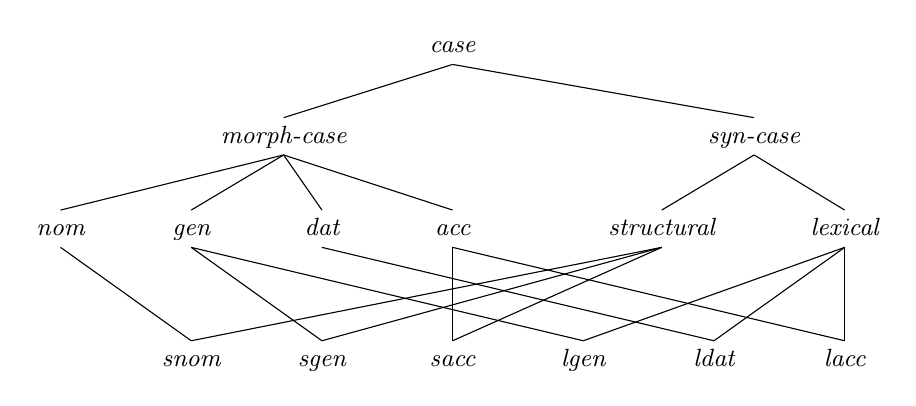
\begin{tikzpicture}[text height=1.5ex,text depth=.25ex,
  % inner sep=2pt,
  node distance=5em,
  baseline=10.75em]\small\it
\node (snom) {snom};
\node (sgen) [right of=snom] {sgen};
\node (sacc) [right of=sgen] {sacc};
\node (lgen) [right of=sacc] {lgen};
\node (ldat) [right of=lgen] {ldat};
\node (lacc) [right of=ldat] {lacc};
\node (acc) [above of=sacc] {acc};
\node (dat) [left of=acc] {dat};
\node (gen) [left of=dat] {gen};
\node (nom) [left of=gen] {nom};
\node (structural) [above of=lgen, xshift=3em] {structural};
\node (lexical) [above of=lacc] {lexical};
\node (morph-case) [above right of=gen] {morph-case};
\node (syn-case) [above right of=structural] {syn-case};
\node (case) [above of=acc, node distance=7em] {case};
\draw (case.south) -- (morph-case.north);
\draw (case.south) -- (syn-case.north);
\draw (morph-case.south) -- (nom.north);
\draw (morph-case.south) -- (gen.north);
\draw (morph-case.south) -- (dat.north);
\draw (morph-case.south) -- (acc.north);
\draw (syn-case.south) -- (structural.north);
\draw (syn-case.south) -- (lexical.north);
\draw (nom.south) -- (snom.north);
\draw (gen.south) -- (sgen.north);
\draw (gen.south) -- (lgen.north);
\draw (dat.south) -- (ldat.north);
\draw (acc.south) -- (sacc.north);
\draw (acc.south) -- (lacc.north);
\draw (structural.south) -- (snom.north);
\draw (structural.south) -- (sgen.north);
\draw (structural.south) -- (sacc.north);
\draw (lexical.south) -- (lgen.north);
\draw (lexical.south) -- (ldat.north);
\draw (lexical.south) -- (lacc.north);
\end{tikzpicture}
\caption{Case hierarchy for German encoding the structural/lexical distinction}
\label{fig:case:germ}
\end{figure}

% \begin{examples}
% \item
% \attop{ 
%   \hspace*{2em}\makebox[28em][c]{{
%       \footnotesize
%       \it
%       \setlength{\unitlength}{0.17ex}
%       \thinlines
%       \begin{picture}(600,250)(-300,-100)
%                                 %
%         \put(0,100){\makebox(0,0){case}}
%         \put(-150,50){\makebox(0,0){morph-case}}
%         \put(150,50){\makebox(0,0){syn-case}}
%         \put(0,90){\line(5,-1){120}}
%         \put(0,90){\line(-5,-1){120}}
%                                 %\bezier{148}(0,90)(145,70)(145,60)
%                                 %\bezier{148}(0,90)(-145,70)(-145,60)
%                                 %
%         \put(70,-10){\makebox(0,0){structural}}
%         \put(210,-10){\makebox(0,0){lexical}}
%         \put(150,40){\line(3,-2){60}}
%         \put(150,40){\line(-2,-1){80}}
%                                 %\bezier{95}(150,40)(210,10)(210,0)
%                                 %\bezier{95}(150,40)(70,10)(70,0)
%                                 %
%         \put(-270,-10){\makebox(0,0){nom}}
%         \put(-190,-10){\makebox(0,0){gen}}
%         \put(-110,-10){\makebox(0,0){dat}}
%         \put(-30,-10){\makebox(0,0){acc}}
%         \put(-150,40){\line(-3,-1){120}}
%         \put(-150,40){\line(3,-1){120}}
%         \put(-150,40){\line(-1,-1){40}}
%         \put(-150,40){\line(1,-1){40}}
%                                 %\bezier{103}(-150,40)(-270,10)(-270,0)
%                                 %\bezier{60}(-150,40)(-190,10)(-190,0)
%                                 %\bezier{60}(-150,40)(-110,10)(-110,0)
%                                 %\bezier{103}(-150,40)(-30,10)(-30,0)
%                                 %
%         \put(-170,-70){\makebox(0,0){snom}}
%         \put(-90,-70){\makebox(0,0){sgen}}
%         \put(-30,-70){\makebox(0,0){sacc}}
%         \put(-270,-20){\line(5,-2){100}}
%         \put(-190,-20){\line(5,-2){100}}
%         \put(-30,-20){\line(0,-2){40}}
%                                 %
%         \put(210,-70){\makebox(0,0){lacc}}
%         \put(130,-70){\makebox(0,0){ldat}}
%         \put(50,-70){\makebox(0,0){lgen}}
%         \put(-190,-20){\line(6,-1){240}}
%         \put(-110,-20){\line(6,-1){240}}
%         \put(-30,-20){\line(6,-1){240}}
%                                 %
%         \put(210,-20){\line(-4,-1){160}}
%         \put(210,-20){\line(-2,-1){80}}
%         \put(210,-20){\line(0,-1){40}}
%                                 %
%         \put(70,-20){\line(-6,-1){240}}
%         \put(70,-20){\line(-4,-1){160}}
%         \put(70,-20){\line(-5,-2){100}}
%                                 %
%       \end{picture}
%       }
%     }
% }
% \zl

Particular verbs may assign specific lexical cases to their arguments, e.g., \ftype{ldat}.  They may also specify arguments as bearing structural case, in which case only the \ftype{str}(\ftype{uctural}) supertype is mentioned in the lexicon.  For example, the lexical entries for \textsc{unterstützen} `support’ and \textsc{helfen} `help’ contain the following subcategorisation requirements:
\eal
\label{ex:hmsubcats}
\ex \textsc{unterst\"utzen}: [\path{subcat}~\sliste{ NP[\type{str}], NP[\type{str}] }] 
\ex \textsc{helfen}: [\path{subcat}~\sliste{ NP[\type{str}], NP[\type{ldat}] }]
\zl
Assuming a~similar \ftype{case} hierarchy for \ili{Icelandic}, the difference between the usual verbs, such as \textsc{elska} `love’ in~\aref{isl:nom}, and “quirky” subject verbs, such as \textsc{vanta} `lack’ in~\rref{isl:acc}, could be represented as below (omitting non-initial arguments):
\eal
\label{ex:islsubcats}
\ex \textsc{elska}: [\path{subcat}~\sliste{ NP[\type{str}], \ldots }] 
\ex \textsc{vanta}: [\path{subcat}~\sliste{ NP[\type{lacc}], \ldots }]
\zl
Since \citet{Pollard94a} and \citet{HM94a}, such representations of case requirements are generally adopted in HPSG,\footnote{A~recent example being \citet[169]{MyPF2018a}.} with the only difference that \path{subcat} is currently replaced with \path{arg-st}.  The point where different approaches diverge is how exactly structural case is resolved to a~specific morphological case.

The simplest principle would resolve the case of the first \ftype{str} argument of a~pure (non-gerundial) verb to nominative, i.e., to \ftype{snom}, the case of any subsequent \ftype{str} argument of a~pure verb to accusative, i.e., to \ftype{sacc}, and the case of any \ftype{str} argument of a~gerund to \ftype{sgen}.  Unfortunately, this simple principle would not work in various cases of raising, e.g., in the case of the \ili{Icelandic} data above.  While the “quirky” cases in~\rref{isl:acc}–\rref{isl:gen} would be properly taken care of by this approach – once the subject is assigned a~specific lexical case it is outside of the realm of a~principle resolving structural cases – structural subjects raised to a~higher verb would be assigned specific case twice (or more times, in the case of longer raising chains): on the \path{subcat} (or \path{arg-st}) of the lower verb and on the \path{subcat} (or \path{arg-st}) of the raising verb.  This would not necessarily lead to problems in the case of raising to subject verbs, as in~\aref{isl:nom}, as the structural argument would be the subject in both subcategorisation frames, so it would be resolved to \ftype{snom} twice, but it would create a~problem in the case of raising to object verbs, as in~\bref{isl:nom}, as the raised argument would be resolved to the nominative on the lower subcategorisation frame and to the accusative on the higher frame.  So, the problem is not limited to \ili{Icelandic}, but may be observed in any language with raising to object (also known as Exceptional Case Marking or Accusativus cum Infinitivo or AcI), including \ili{German} (cf., e.g., \citealt[231]{HM94a}).  Obviously, even if a~structural argument occurs on a~number of \path{subcat} or \path{arg-st} lists, it should be assigned specific morphological case according to its position on just one of them – the highest one.

Both \citet{Pollard94a} and \citet{HM94a} account for such facts via configurational case principles, e.g.~\citep[209]{HM94a}:
\ea\label{hm:cp}
  \princ{Case Principle} (for \ili{German}): \\ [1.5ex]
  In a \ftype{head-complement-structure} whose head has category \\
  \begin{tabular}{ll}
    \ftype{verb\textnormal{[}fin\textnormal{]}} & the external argument has
    a \path{case} value of \ftype{snom}, \\
    \ftype{verb} & the internal argument has a \path{case} value of
    \ftype{sacc}, \\
    \ftype{noun} & the internal argument has a \path{case} value of
    \ftype{sgen}.
  \end{tabular} \\
  These are the only saturated or almost saturated
  \ftype{head-complement-structure}s with structural arguments.
\z
\ea \label{hm:ea}
  \notion{Syntactically External Argument} (`\textit{Subject}'): \\ [1.5ex]
  If the first element of the \path{subcat} list of a sign is an
  NP[\ftype{str}], it is called the (\textit{syntactically}) \notion{external
    argument} of that sign.
\z
\ea \label{hm:ia}
  \notion{Syntactically Internal Argument} (`\textit{Direct Object}'): \\ [1.5ex]
  If the second element of the \path{subcat} list of a sign is an
  NP[\ftype{str}], it is called the (\textit{syntactically}) \notion{internal
    argument} of that sign.
\z
\citet[209–210]{HM94a} formalize this \princ{Case Principle} by
giving the following constraints:
\ea \label{ex:cons:snom}
\onems[phrase]{
synsem|loc|cat \ms{ head & \ms[verb]{
                         vform & fin
                         }\\
                    subcat & \eliste
                  }\\
dtrs \ms[h-c-str]{
     head-dtr|\ldots|subcat & \sliste{ NP[\type{str}], \ldots }\\
     }
} \impl\\
  \hspace*{\fill}
  \ms{
    dtrs$|$head-dtr$|$\ldots$|$subcat & \sliste{ NP[\type{snom}], \ldots } }
\z
\ea
\label{ex:cons:sacc}
\onems[phrase]{
synsem|loc|cat \ms{ head & \ms[verb]{
                         vform & fin
                         }\\
                    subcat & \eliste\ $\vee$ \sliste{ \type{synsem} }
                  }\\
dtrs \ms[h-c-str]{
     head-dtr|\ldots|subcat & \sliste{ \type{synsem}, NP[\type{str}], \ldots }\\
     }
} \impl\\
  \hspace*{\fill}
  \ms{
    dtrs$|$head-dtr$|$\ldots$|$subcat & \sliste{ \type{synsem}, NP[\type{sacc}]}, \ldots }
\z
\ea
\onems[phrase]{
synsem|loc|cat \ms{ head & noun\\
                    subcat & \eliste\ $\vee$ \sliste{ \type{synsem} }
                  }\\
dtrs \ms[h-c-str]{
     head-dtr|\ldots|subcat & \sliste{ \type{synsem}, NP[\type{str}], \ldots }\\
     }
} \impl\\
  \hspace*{\fill}
  \ms{
    dtrs$|$head-dtr$|$\ldots$|$subcat & \sliste{ \type{synsem}, NP[\type{sgen}]}, \ldots }
\z
Note that the locus of this \princ{Case Principle} is \ftype{phrase} and that it makes reference to \ftype{head-complement-structure} values of the \path{daughters} (\path{dtrs}) attribute.  In this sense, this principle is configurational.  Similar principles were proposed for \ili{Korean} \citep{Yoo93a-u,brat:96}, \ili{English} \citep{Grover95a-u} and \ili{Polish} \citep{prze:95b}, \emph{inter alia}.

This configurational approach to case assignment is criticised in \citet{prze:96,Prze99b,Prze99} on the basis of conceptual and theory-internal problems.  The conceptual problem is that a~configurational analysis is employed for what is usually considered an essentially local phenomenon, one concerned with the relation between a~head and its dependents \citep{blak:94}.  The – more immediate – theory-internal problem is that such configurational case principles are restricted to locally realised arguments, and are not necessarily compatible with those – dominant since \citet[Chapter~9]{ps2} – HPSG analyses of extraction which do not assume traces and with those HPSG approaches to cliticisation in which the clitic is realised as an affix rather than a~tree-configurational constituent (cf., e.g., \citealt{MS97a-u} on \ili{French} and \citealt{Monachesi99a-u} on \ili{Italian}).

The solution proposed in \citet{prze:96,Prze99b,Prze99} is to resolve structural cases directly within \path{arg-st}, via local principles operating at the level of \ftype{category} of a~word (where both head information and argument structure information – but not constituent structure – are available) rather than at the level of \ftype{phrase}.  This seems to bring back the problem, discussed in connection with the \ili{Icelandic} data above, of raised arguments, which occur on a~number of \path{arg-st} lists.  The innovation of \citet{prze:96,Prze99b,Prze99} is the proposal to mark, within \textsc{arg-st}, whether a~given argument is realised locally (either tree-con\-fi\-gu\-ra\-tio\-nal\-ly, or as a~gap to be extracted higher on, or as an affix) or not.  If it is realised locally, it may be assigned appropriate case; if it is not (because it is raised), its structural case must be resolved higher up.  On this setup, the above constraints \rref{ex:cons:snom}–\rref{ex:cons:sacc} responsible for the assignment of structural nominative and accusative are replaced with the following two constraints (and similarly for the structural genitive):\footnote{The antecedents of such principles could be further constrained to apply to \ftype{word}s only. As usual, `$\oplus$' indicates concatenation of lists.}
\ea
\label{nonc:cp:germ1}
\ms{
    head & verb \\
    arg-st & \liste{ \ms{ arg NP[\type{str}] \\
                          realized $+$} } $\oplus$ \ibox{2}}
  \impl 
  \ms{
    arg-st \liste{ \ms{ arg  NP[\type{snom}] }} $\oplus$ \ibox{2}} 
\z
\ea \label{nonc:cp:germ2}
\ms{
    head & verb \\
    arg-st & \ibox{1} \type{nelist} $\oplus$ \liste{ \ms{ arg NP[\type{str}] \\
                          realized $+$} } $\oplus$ \ibox{2}}
  \impl\\ 
  \ms{
    arg-st \ibox{1} $\oplus$ \liste{ \ms{ arg  NP[\type{snom}] }} $\oplus$ \ibox{2}} 
\z
Obviously, for such constraints to work, values of \path{arg-st} must be lists of slightly more complex objects than \ftype{synsem} (these are now values of \path{arg} within such more complex objects), and additional principles must make sure that values of \path{realized} are instantiated properly (see \citealt[78–79]{Prze99b} for details).

% While this approach seems to be sufficient to account for almost all known structural case phenomena, German presents additional difficulties, as discussed in \citealt{Mueller97d,Mueller2001a-cr} and \citealt{Meurers99c,Meurers99b}.  In brief, \citet{Mueller97d,Mueller2001a-cr} recalls arguments from \citealt{Hoehle83a,HoehleTopo} that, in German, controlled (not:~raised) structural subjects bear the nominative case.  Since such subjects are never realised locally (as such), the above case principle stated in terms of \path{realized} would not resolve their case.  The problem with the particular approach of \citealt{prze:96,Prze99b,Prze99} is the assumption that an argument is locally realised – and hence may be assigned structural case – if and only if it is not raised to a~higher argument structure.  The kind of data discussed in \citealt{Hoehle83a,HoehleTopo} and \citealt{Mueller97d,Mueller2001a-cr} shows that this equivalence does not always hold and suggests that structural case should be assigned to arguments on the basis of whether they are raised or not, and not whether they are locally realised or not.

The analysis of \citet{prze:96,Prze99b,Prze99} assumes that an argument is locally realised – and hence may be assigned structural case – if and only if it is not raised to a~higher argument structure.  \citet{Meurers99c,Meurers99b}, on the basis of empirical observations in \citet{Haider90a}, \citet{Grewendorf94a} and \citet{Mueller97c-Eng}, shows that this assumption does not always hold in \ili{German}; rather, structural case should be assigned to arguments on the basis of whether they are raised or not, and not whether they are locally realised or not.  Consider the following data \citep[294]{Meurers99c}:
\eal
\ex\label{win:ss}
\gll [\emph{Ein} \emph{Außenseiter} gewinnen] wird hier nie. \\
    \phtm{[}an.\NOM{} outsider win.\INF{} will here never\\
\glt `An outsider will never win here.'
\ex\label{win:so}
\gll [\emph{Einen} \emph{Außenseiter} gewinnen] läßt Gott hier nie. \\
    \phtm{[}an.\ACC{} outsider win.\INF{} lets god here never\\
\glt `God never lets an outsider win here.'
\zl
Assuming that fronted fragments, marked with square brackets, are single constituents,\footnote{This assumption is not completely uncontroversial; see \citet[100–101]{Kiss94} for apparent counterexamples and \citet{Mueller2003b,Mueller2005d,MuellerGS} for a defense of this assumption.} the subject of \emph{gewinnen} `win’ forms a~constituent with this verb, i.e., it has the same configurational realisation in both examples.  Hence, configurational case assignment principles should assign it the same case in both instances, contrary to facts: \emph{ein Au\ss{}enseiter} occurs in the nominative in~\rref{win:ss} and \emph{einen Au\ss{}enseiter} bears the accusative case in~\rref{win:so}.  As argued by \citet{Meurers99c,Meurers99b}, the reason is that – although the subject is realised locally to its infinitival head – it is in some sense raised further to the subject position of the auxiliary \emph{wird} in~\rref{win:ss} and to the object position of the AcI verb \emph{l\"a\ss{}t} in~\rref{win:so}, hence the difference in cases.  This suggests that structural case should be assigned not where the argument is realised, but on the highest \path{arg-st} on which it occurs.  A~corresponding modification of the non-configurational case assignment approach of \citet{prze:96,Prze99b,Prze99} – replacing the [\path{realized}~$+$] with [\path{raised}~$-$] in constraints such as~\rref{nonc:cp:germ1}–\rref{nonc:cp:germ2} and providing appropriate constraints on values of \path{raised} – is proposed in~\citet[93–95]{Prze99b}; see also \citet{MuellerLehrbuch3}, Section~17.4 (and references therein) for further improvements.

While this non-configurational approach to syntactic case assignment was motivated largely by the need to capture complex interactions in a~precise way, it turns out to formalise sometimes apparently contradictory intuitions expressed in various approaches to case.  First of all, it preserves the common intuition that case is a~local phenomenon, an intimate relation between a~head and its dependents.  Second, it successfully formalises the distinction between structural and inherent/lexical case known from the transformational literature of the 1980s, and non-configurationally encodes the apparently configurational principles of structural case assignment.  Third, while most HPSG literature on case is concerned with syntactic phenomena in European languages, this approach has been extended to case stacking known, e.g., from languages of Australia and case attraction observed, e.g., in \ili{Classical Armenian} and in \ili{Gothic} \citep{malo:00}.  Fourth, by allowing antecedents of implicational constraints such as \rref{nonc:cp:germ1}–\rref{nonc:cp:germ2} to be \ftype{local} objects, not just syntactic \ftype{categories}, semantic factors influencing case assignment may also be taken into account, as in differential case marking, repeatedly considered in \is{Lexical Functional Grammar|(}Lexical Functional Grammar (cf., e.g., \citealt{BHK2003a-u} and references therein), but apparently not (so far) in HPSG\@.  Fifth, as pointed out in \citet{Prze99b,Prze99}, the above approach to case formalises the “case tier” intuition of \citet{ZMT85a}, \citet{YMJ87} and \citet{mali:93} (see also \citealt{mali:09}).

Let us illustrate the last point with some \ili{Finnish} data from~\citet{mali:93}:
\eal
\label{subj}
\ex \gll Liisa muisti matkan vuoden. \\
    Liisa.\NOM{} remembered trip.\ACC{} year.\ACC{}\\
\glt  `Liisa remembered the trip for a year.'
\ex
\label{adv1bis}\label{obj}
\gll Lapsen täytyy lukea kirja \phtm{[}kolmannen kerran. \\
    child.\GEN{} must read book.\NOM{} [third time].\ACC{}\\
\glt  `The child must read the book for a third time.'
\ex
\label{adv1}
\gll Kekkoseen luotettiin \phtm{[}yksi kerta. \\
    Kekkonen\Ill{} trust\PassP{} [one time].\NOM{}\\
\glt `Kekkonen was trusted once.'
\ex
\label{adv2}
\gll Kekkoseen luotettiin \phtm{[}yhden kerran \phtm{[}yksi vuosi. \\
    Kekkonen\Ill{} trust\PassP{} [one time].\ACC{} [one year].\NOM{}\\
\glt  `Kekkonen was trusted for one year once.'
\zl
\citet{mali:93} argues at length that some adjuncts (adverbials of measure,
duration and frequency) behave just like objects with respect to case
assignment and, in particular, notes the following generalization about
syntactic case assignment: only one NP dependent of the verb receives the
nominative, namely the one which has the highest grammatical function;
other dependents receive the accusative.\footnote{See also
  \citet{zae:mal:83} and \citet{ZMT85a} for a similar generalisation with respect to
  \ili{Icelandic}.}  Thus, if none of the arguments bears inherent case, the
subject is in the nominative and other dependents are in the accusative, cf.~\rref{subj}, but if the subject bears an idiosyncratic case, it is the
object that gets the nominative, cf.~\rref{obj}.  Furthermore, if all arguments
(if any) bear inherent case, the next “available” grammatical function is
that of an adjunct, thus one of the adjuncts receives the nominative, 
cf.~\rref{adv1}–\rref{adv2}.

Given such facts,
\citet{mali:93} claims that syntactic case is assigned in \ili{Finnish} on
the basis of grammatical hierarchy and that (at least some) adjuncts
belong to this hierarchy.  Moreover, as evidenced by
\rref{adv1}–\rref{adv2}, adjuncts do not form a single class in this
hierarchy: although the multiplicative adverbial \emph{yksi kerta} is
nominative in \rref{adv1}, this case is won over by the duration
adverbial in \rref{adv2}. Taking into consideration also the partitive
of negation facts (measure adverbials, but not duration or frequency
adverbials, behave like direct objects in the sense that they take
partitive case under sentential negation), \citet{mali:93} extends the
grammatical function hierarchy for \ili{Finnish} in the following way:
\eal
SUBJ $>$ OBJ $>$ MEASURE $>$ DURATION $>$ FREQUENCY
\zl

While these generalisations are developed in the context of Lexical Functional Grammar, it is not clear how they could be encoded in LFG: there are no formal mechanisms for stating such a~hierarchy of grammatical functions and, additionally, all adjuncts are assumed to be elements of an unordered set.\footnote{But see \citet{Prze2016a} for an attempt to introduce a~single ordered list of dependents and formalise the functional hierarchy in LFG\@.}\is{Lexical Functional Grammar|)}  On the other hand, given the “adjuncts as complements” approach of \citet{BMS2001a-unlinked} and others, upon which at least some adjuncts are added to \path{arg-st} (perhaps renamed to \path{deps}), and assuming – as is standard in HPSG – that \path{arg-st} elements satisfy the obliqueness hierarchy, formalisation of the “case tier” approach is easy and consists of two implicational principles similar to \rref{nonc:cp:germ1}–\rref{nonc:cp:germ2}.  The first principle resolves the first structurally-cased element of extended \path{arg-st} to nominative, whether this element is the first element of \path{arg-st} or not (it is not in the case of \rref{obj}–\rref{adv2}), and whether it corresponds to the subject, the direct object or an adjunct.  The second principle resolves the structural case of all subsequent elements, if any, to accusative.






\section{Case syncretism and neutrality}
\label{sec:case:syn}

Another important strand of HPSG work on case concerns situations in which a~single syncretic form seems to simultaneously bear two (or more) case values, as in the following examples involving \isi{coordination}, \isi{free relatives} and \isi{parasitic gaps}:
\begin{exe} 
\ex
\label{ex:syn:pc} \ili{Polish} coordination \citep[701–702]{Dyla84}:
\begin{xlist}
\ex[]{
\gll Kogo Janek lubi a Jerzy nienawidzi? \\
      who.\textsc{acc/gen} Janek.\textsc{nom} likes(\textsc{obj.acc}) and Jerzy.\textsc{nom} hates(\textsc{obj.gen})\\
\glt `Who does Janek like and Jerzy hate?’
}
\ex[*]{
\gll Co Janek lubi a Jerzy nienawidzi? \\
      what.\textsc{nom/acc} Janek.\textsc{nom} likes(\textsc{obj.acc}) and Jerzy.\textsc{nom} hates(\textsc{obj.gen})\\
\glt Intended: `What does Janek like and Jerzy hate?’
}
\zl
\ea
\label{ex:syn:ec} \ili{English} coordination (\citealt[70]{Goodall87a-u}; \citealt[206]{LHC2001a-u}): \\ [1ex]
  This is the man who$_i$.\textsc{nom/acc} Robin saw $e_i$.\textsc{acc} and thinks $e_i$.\textsc{nom} is handsome.
\z
\begin{exe}
\ex \label{ex:syn:gc}
\ili{German} coordination \citep[764–765]{PZ86}:
\begin{xlist}
\ex[]{
\gll  Er findet und hilft Frauen. \\
      he.\textsc{nom} finds(\textsc{obj.acc}) and helps(\textsc{obj.dat}) women.\textsc{nom/acc/gen/dat}\\
\glt `He finds and helps women.’
}
\ex[*]{
\gll  Sie findet und hilft Männer. \\
      she.\textsc{nom} finds(\textsc{obj.acc}) and helps(\textsc{obj.dat}) men.\textsc{nom/acc/gen}\\
\glt Intended: `She finds and helps men.’
}
\ex[*]{
\gll  Sie findet und hilft Männern. \\
      she.\textsc{nom} finds(\textsc{obj.acc}) and helps(\textsc{obj.dat}) men.\textsc{dat}\\
\glt Intended: `She finds and helps men.’
}
\zl
\ea\label{ex:syn:gfr} 
\ili{German} free relatives \citep[212]{GR81}: \\ [1ex]
\gll Was du mir gegeben hast, ist prächtig. \\
     what.\textsc{nom/acc} you.\textsc{nom} me.\textsc{dat} given(\textsc{obj.acc}) have is(\textsc{subj.nom}) wonderful\\
\glt `What you have given to me is wonderful.’
\z
\ea
\label{ex:syn:epg}
\ili{English} parasitic gaps (\citealt[482]{HL96a}; \citealt[205]{LHC2001a-u}): \\[1ex]
  Robin is someone who$_i$.\textsc{nom/acc} even good friends of $e_i$.\textsc{acc} believe $e_i$.\textsc{nom} should be closely watched.
\z
In~\aref{ex:syn:pc}, the fronted syncretic accusative/genitive form \emph{kogo} `who’ satisfies the requirements of the two coordinated verbal constituents: in one, \emph{lubi} `likes’ requires an accusative object, and in the other, \emph{nienawidzi} `hates’ expects a~genitive object.  A~form which is not syncretic between (at least) these two cases cannot occur in the place of \emph{kogo}; this is illustrated in~\bref{ex:syn:pc}, where the element putatively shared by the two verbal constituents is syncretic between accusative and nominative, rather than accusative and genitive.  The \ili{English} example~\rref{ex:syn:ec} is similar and involves the relative pronoun \emph{who}, syncretic between accusative and nominative.  The well-known example~\rref{ex:syn:gc} illustrates essentially the same phenomenon in \ili{German}: the form \emph{Frauen} `women’, which is fully syncretic with respect to case, simultaneously satisfies the accusative requirement of \emph{findet} `finds’ and the dative requirement of \emph{hilft} `helps’.  By contrast, this joint requirement is not satisfied either by \emph{Männer}, which is accusative (among other cases) but not dative, or by \emph{Männern}, which is dative but not accusative.  The other two examples show that this phenomenon is not restricted to coordination.  In~\rref{ex:syn:gfr}, the syncretic form \emph{was} `what’ simultaneously satisfies the constraint that the object of \emph{gegeben} `given’ is accusative and that the subject of \emph{ist} `is’ is nominative.  Similarly, the extracted \emph{who} in~\rref{ex:syn:epg} seems to simultaneously bear the accusative case assigned by the preposition \emph{of} and the nominative case of the subject of \emph{should}.

Such examples were at one point considered problematic not only for HPSG, but for unification-based theories in general \citep{Ingria90}.  The reason is that, on the straightforward approach to case, they should all be ungrammatical.  For example, in the case of \aref{ex:syn:gc}, the assignment of the accusative to the object of \emph{findet} `finds’ should clash with the assignment of the dative to the object of \emph{hilft} `helps’, as both objects are realised by the same noun \emph{Frauen} `women’.  In other words, the attempt to unify accusative and dative should fail.  

The solution first proposed by \citet[207–208]{LHC2001a-u} is to enrich the \ftype{case} hierarchy
in such a~way that the unification of two different morphological cases does not necessarily result
in failure.\footnote{See \citet[196]{Ingria90} for an earlier implementation of roughly the same
  idea in the context of unification grammars.}  Specifically, assuming that nominative and
accusative are structural cases in \ili{English}, they propose the part of the structural
case hierarchy shown in Figure~\ref{fig:daniels18}.\footnote{Type names follow the convention in \citet{dani:01}, for increased uniformity with the remainder of this section.}
%\pagebreak
\begin{figure}
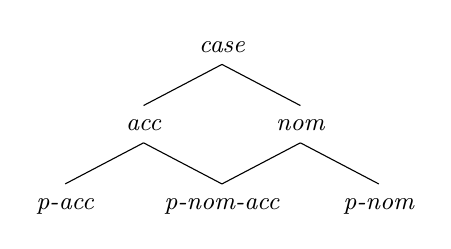
\begin{tikzpicture}[text height=1.5ex,text depth=.25ex,
  % inner sep=2pt,
  node distance=3em,
  baseline=5.25em]\small\it
\node (p-acc) {p-acc};
\node (p-acc1) [right of=p-acc] {};
\node (p-nom-acc) [right of=p-acc1] {p-nom-acc};
\node (p-nom1) [right of=p-nom-acc] {};
\node (p-nom) [right of=p-nom1] {p-nom};
\node (acc) [above of=p-acc1] {acc};
\node (nom) [above of=p-nom1] {nom};
\node (p-nom-acc1) [above of=p-nom-acc] {};
\node (case) [above of=p-nom-acc1] {case};
\draw (case.south) -- (acc.north);
\draw (case.south) -- (nom.north);
\draw (acc.south) -- (p-acc.north);
\draw (acc.south) -- (p-nom-acc.north);
\draw (nom.south) -- (p-nom.north);
\draw (nom.south) -- (p-nom-acc.north);
\end{tikzpicture}
% \mbox{}\\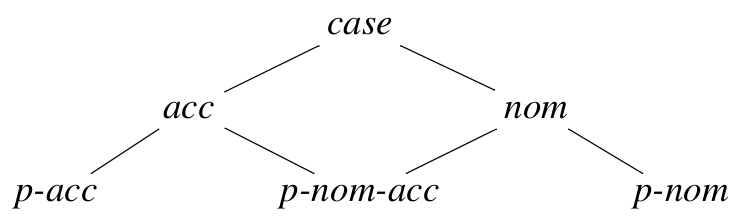
\includegraphics[scale=.35]{daniels18.png}
\caption{Case hierarchy for English encoding case syncretism}\label{fig:daniels18} 
\end{figure}
% \begin{verbatim}
%              scase
%             /     \
%         snom       sacc
%        /    \     /    \
%     nom     nom_acc     acc
% \end{verbatim}

Particular nominal forms are specified in the lexicon as either pure accusative (\ftype{p-acc}), pure nominative (\ftype{p-nom}) or syncretic between the two (\ftype{p-nom-acc}):
\ea
  \begin{tabular}[t]{ll}
  \emph{he} & [\path{case}~\ftype{p-nom}] \\
  \emph{him} & [\path{case}~\ftype{p-acc}] \\
  \emph{whom} & [\path{case}~\ftype{p-acc}] \\
  \emph{who} & [\path{case}~\ftype{p-nom-acc}] \\
  \emph{Robin} & [\path{case}~\ftype{p-nom-acc}] \\
  \end{tabular}
\z
On the other hand, heads – or constraints of a~case principle of the kind presented in the previous section – specify particular arguments as \ftype{nom} or \ftype{acc}.  So, in the case of the parasitic gap example~\rref{ex:syn:epg}, the \ftype{acc} requirement associated with the preposition \emph{of} and the \ftype{nom} requirement on the subject of \emph{should} are not incompatible: their unification results in \ftype{p-nom-acc} and the shared dependent may be any form compatible with this case value, e.g., \emph{who} (but not \emph{whom}).  Examples~\rref{ex:syn:pc}–\rref{ex:syn:gfr} can be handled in a~similar way.

A~situation often perceived as dual to such case neutrality, sometimes called “case underspecification”, occurs when a~head specifies the case of its dependent disjunctively and may combine with a~\is{coordination|(}coordinate structure containing phrases in both cases, e.g.:
\eal
\ex\label{ex:dis:pl}
\ili{Polish} \citep[175]{Prze99b}: \\ [1ex]
\gll Dajcie wina i całą świnię! \\
    give wine.\GEN{} and whole.\ACC{} pig.\ACC{}\\
\glt `Serve (some) wine and a whole pig!’
\ex\label{ex:dis:ru} \ili{Russian} \citep[11]{levy:01}: \\ [1ex]
\gll V{\v c}era vec' den' on pro{\v z}dal svoju podrugu Irinu i zvonka ot svoego brata Grigorija. \\
    yesterday all day he expected self's.\ACC{} girlfriend.\ACC{} Irina.\ACC{} and call.\GEN{} from self's brother Grigory\\
\glt `Yesterday he waited all day for his girlfriend Irina and for a~call from his brother Grigory.’
\zl
In \ili{Polish}, the object of the verb \emph{dajcie} `give’ is normally in the accusative, but may also be realised as the genitive, when its meaning is partitive; in~\rref{ex:dis:pl}, the object is a~coordination of such a~genitive noun \emph{wina} `(some) wine’ and the accusative \emph{całą świnię} `whole pig’.  Similarly, according to \citealt{levy:01}, the \ili{Russian} verb \emph{pro{\v z}dal} `awaited’ may combine with accusative or genitive, and in~\rref{ex:dis:ru} it happily combines with a~coordinate phrase containing both.

If such “accusative and genitive” coordinate phrases bear case at all, the value of this grammatical category must be something like \ftype{acc+gen}.  Note that this situation differs from case neutrality discussed above: a~syncretic case such as \ftype{p-acc-gen} intuitively corresponds to intersection: a~nominal bearing this case is accusative and genitive at the same time.  On the other hand, the intuition behind \ftype{acc+gen} is that of union: a~(coordinated) nominal with this case value has accusative elements and genitive elements, so it may fill a~position disjunctively specified as requiring accusative \emph{or} genitive.  However, \ftype{acc+gen} coordinate phrases cannot fill either purely accusative positions (because such phrases contain genitive – i.e., non-accusative – conjuncts), or purely genitive positions (because of accusative – i.e., non-genitive – conjuncts), or positions simultaneously specified as accusative \emph{and} genitive, as in~\rref{ex:syn:pc} above (for both reasons).

This duality is a~feature of the \isi{Categorial Grammar} approach to case and coordination of \citet{Bayer96} (see also \citealt{BJ95}) and the corresponding HPSG analyses were presented in \citet{levy:01} and \citet{lev:pol:01}, as well as in~\citet{dani:01}.  As noted in~\citet[233]{lev:pol:01}, the two HPSG approaches are isomorphic.  The main technical difference is that the relevant case hierarchies are construed outside of the usual HPSG type hierarchy in the approach of \citet{levy:01} and \citet{lev:pol:01}, but they are fully integrated in the approach of \citet{dani:01}.  For this reason, and also because it is the basis of some further HPSG work (e.g., \citealt{Crysmann2005c}), this latter approach is presented below.

Intuitively, just as the common subtype of \ftype{acc} and \ftype{nom}, i.e., \ftype{p-nom-acc}
in Figure~\ref{fig:daniels18}, represents forms which are simultaneously accusative and nominative, the common
supertype, i.e., \ftype{case}, which should perhaps be renamed to \ftype{nom+acc}, should represent
coordinate structures involving nominative and accusative conjuncts.  However, given that all
objects are assumed to be sort-resolved in standard HPSG, saying that the case of a~coordinate
structure is \ftype{case} (or \ftype{nom+acc}) is paramount to saying that it is either
\ftype{p-acc} (pure accusative), or \ftype{p-nom-acc} (syncretic nominative/accusative), or
\ftype{p-nom} (pure nominative).  One solution is to “make a~simple change to the framework's
foundational assumptions” \citep[268]{sag:02} and to allow linguistic objects to bear non-maximal
types.  This is proposed and illustrated in detail in \citet{sag:02}.  A~more conservative
solution, proposed in \citet{dani:01}, is to add dedicated maximal types to all such non-maximal
types; for example, the hierarchy in Figure~\ref{fig:daniels18} is modified as shown in Figure~\ref{fig:daniels20}.
\begin{figure}
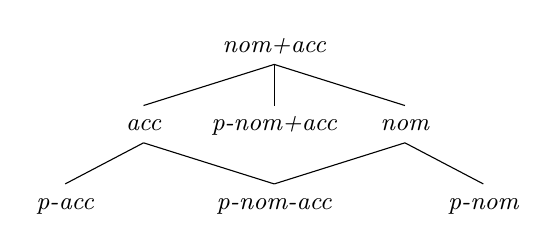
\begin{tikzpicture}[text height=1.5ex,text depth=.25ex,
  % inner sep=2pt,
  node distance=4em,
  baseline=5.25em]\small\it
\node (p-acc) {p-acc};
\node (p-acc1) [right of=p-acc] {};
\node (p-nom-acc) [right of=p-acc1] {p-nom-acc};
\node (p-nom1) [right of=p-nom-acc] {};
\node (p-nom) [right of=p-nom1] {p-nom};
\node (acc) [above of=p-acc1, node distance=3em, xshift=-1em] {acc};
\node (nom) [above of=p-nom1, node distance=3em, xshift=1em] {nom};
\node (p-nom+acc) [above of=p-nom-acc, node distance=3em] {p-nom+acc};
\node (nom+acc) [above of=p-nom+acc, node distance=3em] {nom+acc};
\draw (nom+acc.south) -- (acc.north);
\draw (nom+acc.south) -- (nom.north);
\draw (nom+acc.south) -- (p-nom+acc.north);
\draw (acc.south) -- (p-acc.north);
\draw (acc.south) -- (p-nom-acc.north);
\draw (nom.south) -- (p-nom.north);
\draw (nom.south) -- (p-nom-acc.north);
\end{tikzpicture}
% \mbox{}\\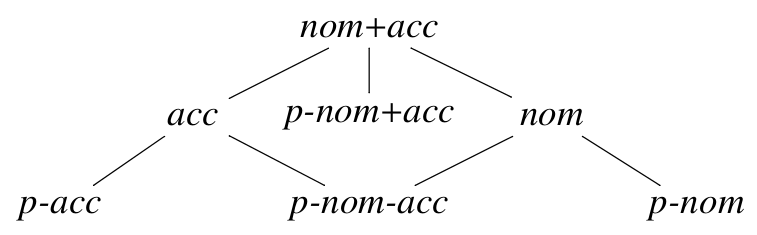
\includegraphics[scale=.35]{daniels20.png}
\caption{Case (sub)hierarchy encoding nominative/accusative syncretism and underspecification}
\label{fig:daniels20} 
\end{figure}
Apart from the trivial renaming of \ftype{case} to the more explicit \ftype{nom+acc}, a~maximal type corresponding to this renamed non-maximal type is added here, namely, \ftype{p-nom+acc}.

Let us illustrate this approach with the two \ili{Polish} examples~\aref{ex:syn:pc} and \rref{ex:dis:pl}, repeated below as \rref{ex:syn:pc:again}–\rref{ex:dis:pl:again}:
\eal
\ex
\label{ex:syn:pc:again} 
\gll Kogo Janek lubi a Jerzy nienawidzi? \\
     who.\textsc{acc/gen} Janek.\textsc{nom} likes(\textsc{obj.acc}) and Jerzy.\textsc{nom} hates(\textsc{obj.gen})\\\hspace{-6pt}
\glt  `Who does Janek like and Jerzy hate?’
\ex\label{ex:dis:pl:again}
\gll Dajcie wina i całą świnię! \\
    give wine.\GEN{} and whole.\ACC{} pig.\ACC{}\\
\glt `Serve (some) wine and a whole pig!’
\zl
As these examples involve accusative and genitive, I will assume that the complete case hierarchy
contains a~subhierarchy such as that in Figure~\ref{fig:daniels20} above, but with all occurrences of
\ftype{nom} replaced by \ftype{gen} as in Figure~\ref{fig:case4}.
\begin{figure}
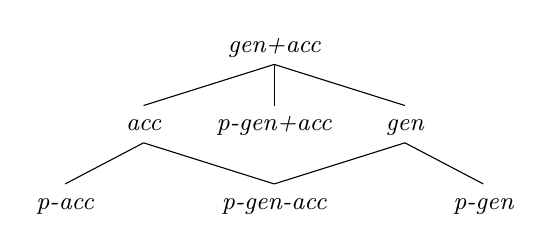
\begin{tikzpicture}[text height=1.5ex,text depth=.25ex,
  % inner sep=2pt,
  node distance=4em,
  baseline=5.25em]\small\it
\node (p-acc) {p-acc};
\node (p-acc1) [right of=p-acc] {};
\node (p-gen-acc) [right of=p-acc1] {p-gen-acc};
\node (p-gen1) [right of=p-gen-acc] {};
\node (p-gen) [right of=p-gen1] {p-gen};
\node (acc) [above of=p-acc1, node distance=3em, xshift=-1em] {acc};
\node (gen) [above of=p-gen1, node distance=3em, xshift=1em] {gen};
\node (p-gen+acc) [above of=p-gen-acc, node distance=3em] {p-gen+acc};
\node (gen+acc) [above of=p-gen+acc, node distance=3em] {gen+acc};
\draw (gen+acc.south) -- (acc.north);
\draw (gen+acc.south) -- (gen.north);
\draw (gen+acc.south) -- (p-gen+acc.north);
\draw (acc.south) -- (p-acc.north);
\draw (acc.south) -- (p-gen-acc.north);
\draw (gen.south) -- (p-gen.north);
\draw (gen.south) -- (p-gen-acc.north);
\end{tikzpicture}
\caption{Case (sub)hierarchy encoding accusative/genitive syncretism and underspecification}\label{fig:case4}
\end{figure}


First of all, heads subcategorise for (or relevant case principles specify) “non-pure” cases, i.e., \ftype{acc}, \ftype{gen}, \ftype{gen+acc}, etc., but not \ftype{p-acc}, \ftype{p-gen}, \ftype{p-gen+acc}, etc.  For example, \emph{lubi} `likes’ and \emph{nienawidzi} `hates’ in~\rref{ex:syn:pc:again} expect their objects to have the case values \ftype{acc} and \ftype{gen}, respectively.  Moreover, \emph{dajcie} `give’ in~\rref{ex:dis:pl:again} specifies the case of its object as \ftype{gen+acc}.  On the other hand, nominal dependents bear “pure” cases.  For example, \emph{kogo} `who’ in~\rref{ex:syn:pc:again} is lexically specified as \ftype{p-gen-acc}.  Similarly to the analysis of the English parasitic gap example above, this neutralised case is compatible with both specifications: \ftype{acc} and \ftype{gen}.

The analysis of~\rref{ex:dis:pl:again} is a~little more complicated, as a~new principle is needed to determine the case of a~coordinate structure.  The two conjuncts, \emph{wina} `wine’ and \emph{całą świnię} `whole pig’, have -- by virtue of lexical specifications of their head nouns -- the case values \ftype{p-gen} and \ftype{p-acc}, respectively.  Now, the case value of the coordination is determined as follows: take the “non-pure” versions of the cases of all conjuncts (here: \ftype{gen} and \ftype{acc}), find their (lowest) common supertype (here: \ftype{gen+acc}), and assign to the coordinate structure the “pure” type corresponding to this common supertype (here: \ftype{p-gen+acc}).  This way the coordinate structure in~\rref{ex:dis:pl:again} ends up with the case value \ftype{p-gen+acc}, which is compatible with the \ftype{gen+acc} requirement posited by the verb \emph{dajcie} (or by an appropriate principle of structural case assignment).  Obviously, a~purely accusative, purely genitive or accusative/genitive neutralised object would also satisfy this requirement.

One often-perceived – both within and outside of HPSG – problem with this approach is that it leads
to very complex type hierarchies for \ftype{case} and rather inelegant constraints
(\citealt[272]{sag:02}, \citealt[63–66]{dal:kin:sad:09}).  Let us, following \citet{dani:01},
simplify the presentation of type hierarchies such as that in Figure~\ref{fig:daniels20}, by removing all those “pure” types which are only needed to represent some
non-maximal types as maximal as in Figure~\ref{fig:daniels21}.
\begin{figure}
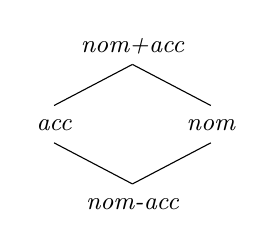
\begin{tikzpicture}[text height=1.5ex,text depth=.25ex,
  % inner sep=2pt,
  node distance=3em,
  baseline=2.5em]\small\it
\node (acc) {acc};
\node (accnom) [right of=acc] {};
\node (nom) [right of=accnom] {nom};
\node (nom-acc) [below of=accnom] {nom-acc};
\node (nom+acc) [above of=accnom] {nom+acc};
\draw (nom+acc.south) -- (acc.north);
\draw (nom+acc.south) -- (nom.north);
\draw (acc.south) -- (nom-acc.north);
\draw (nom.south) -- (nom-acc.north);
\end{tikzpicture}
\caption{Simplified case (sub)hierarchy encoding nominative/accusative syncretism and underspecification}\label{fig:daniels21} 
\end{figure}
Hence, the representation in this figure corresponds to seven types shown explicitly in Figure~\ref{fig:daniels20}
(each non-maximal type in Figure~\ref{fig:daniels21} has an additional \ftype{p-} type, while the maximal
\ftype{nom-acc} in Figure~\ref{fig:daniels21} is the same as \ftype{p-nom-acc} in Figure~\ref{fig:daniels20}).
What would a~similar hierarchy for three morphological cases look like?  \citet[143]{dani:01}
provides the visualisation in Figure~\ref{fig:daniels22}, involving 18 nodes corresponding to 35 types in the full type hierarchy.
%\pagebreak
\begin{figure}
\hfill\hfill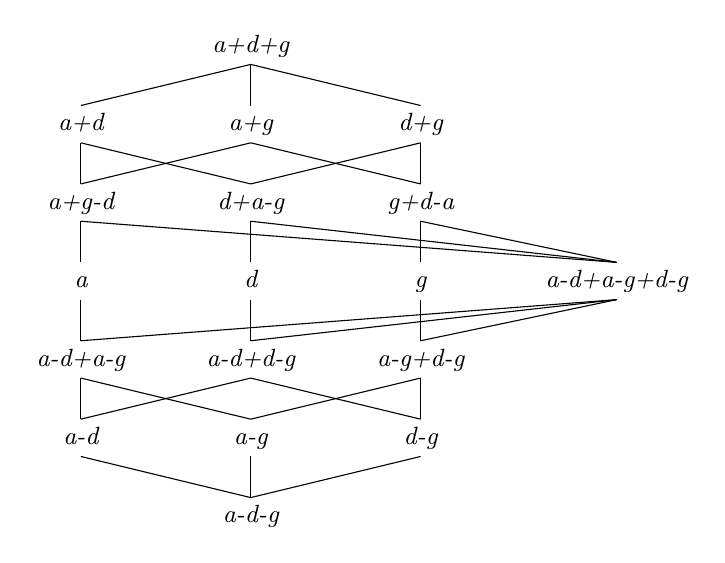
\begin{tikzpicture}[text height=1.5ex,text depth=.25ex,
  % inner sep=2pt,
  node distance=6.5em,
  baseline=8em]\small\it
\node (a) {a};
\node (d) [right of=a] {d};
\node (g) [right of=d] {g};
\node (a-d+a-g+d-g) [right of=g, xshift=1em] {a-d+a-g+d-g};
\node (a+g-d) [above of=a, node distance=3em]  {a+g-d};
\node (d+a-g) [above of=d, node distance=3em] {d+a-g};
\node (g+d-a) [above of=g, node distance=3em] {g+d-a};
\node (a+d) [above of=a+g-d, node distance=3em] {a+d};
\node (a+g) [above of=d+a-g, node distance=3em] {a+g};
\node (d+g) [above of=g+d-a, node distance=3em] {d+g};
\node (a+d+g) [above of=a+g, node distance=3em] {a+d+g};
\node (a-d+a-g) [below of=a, node distance=3em] {a-d+a-g};
\node (a-d+d-g) [below of=d, node distance=3em] {a-d+d-g};
\node (a-g+d-g) [below of=g, node distance=3em] {a-g+d-g};
\node (a-d) [below of=a-d+a-g, node distance=3em] {a-d};
\node (a-g) [below of=a-d+d-g, node distance=3em] {a-g};
\node (d-g) [below of=a-g+d-g, node distance=3em] {d-g};
\node (a-d-g) [below of=a-g, node distance=3em] {a-d-g};
\draw (a+g-d.south) -- (a.north);
\draw (a+g-d.south) -- (a-d+a-g+d-g.north);
\draw (d+a-g.south) -- (d.north);
\draw (d+a-g.south) -- (a-d+a-g+d-g.north);
\draw (g+d-a.south) -- (g.north);
\draw (g+d-a.south) -- (a-d+a-g+d-g.north);
\draw (a+d.south) -- (a+g-d.north);
\draw (a+d.south) -- (d+a-g.north);
\draw (a+g.south) -- (a+g-d.north);
\draw (a+g.south) -- (g+d-a.north);
\draw (d+g.south) -- (d+a-g.north);
\draw (d+g.south) -- (g+d-a.north);
\draw (a+d+g.south) -- (a+d.north);
\draw (a+d+g.south) -- (a+g.north);
\draw (a+d+g.south) -- (d+g.north);
\draw (a.south) -- (a-d+a-g.north);
\draw (d.south) -- (a-d+d-g.north);
\draw (g.south) -- (a-g+d-g.north);
\draw (a-d+a-g.south) -- (a-d.north);
\draw (a-d+a-g.south) -- (a-g.north);
\draw (a-d+d-g.south) -- (a-d.north);
\draw (a-d+d-g.south) -- (d-g.north);
\draw (a-g+d-g.south) -- (a-g.north);
\draw (a-g+d-g.south) -- (d-g.north);
\draw (a-d.south) -- (a-d-g.north);
\draw (a-g.south) -- (a-d-g.north);
\draw (d-g.south) -- (a-d-g.north);
\draw (a-d+a-g+d-g.south) -- (a-d+a-g.north);
\draw (a-d+a-g+d-g.south) -- (a-d+d-g.north);
\draw (a-d+a-g+d-g.south) -- (a-g+d-g.north);
\end{tikzpicture}\hfill\mbox{}
% \\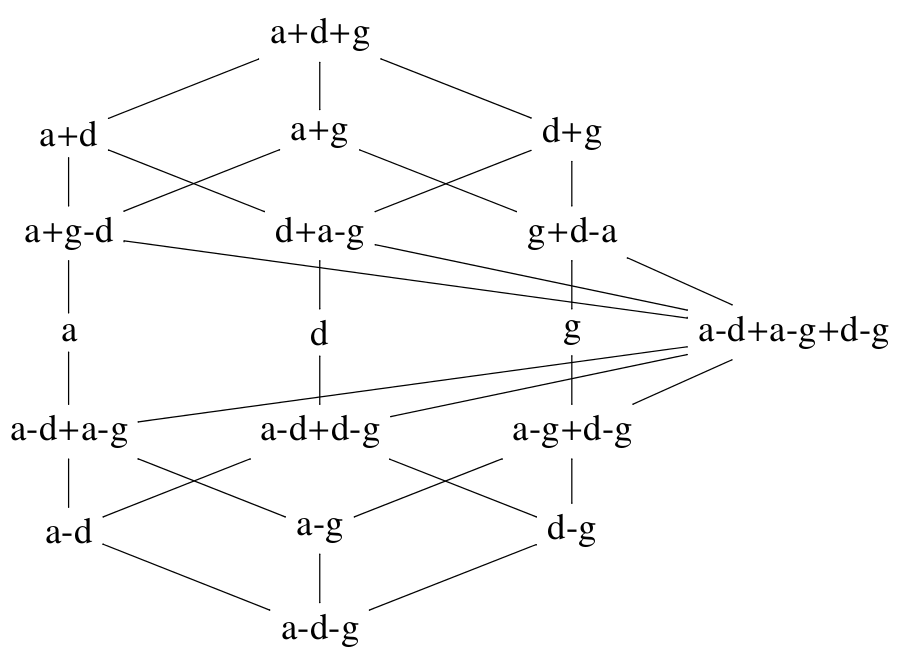
\includegraphics[scale=.35]{daniels22.png}
\caption{Simplified case (sub)hierarchy encoding accusative\slash dative\slash genitive syncretism and underspecification}
\label{fig:daniels22} 
\end{figure}
As mentioned in~\citet[225]{lev:pol:01}, the size of such a~type hierarchy grows double exponentially with the number of grammatical cases, so it would already be next to impossible to visualise such a~hierarchy for German, with its four cases, not to mention Polish with its seven cases or Finno-Ugric languages with around 15 cases.  And matters are further complicated by the fact that sometimes form syncretism simultaneously involves a~number of grammatical categories, so perhaps such type hierarchies should combine case information with person, gender and number (\citealt[145]{dani:01}, \citealt{Crysmann2005c}), and by the fact that coordinated elements may be specified for different categories (e.g., an NP specified for case may be coordinated with a~sentence), in which case it is not clear what categories should be borne by the coordinate structure as a~whole (see, e.g., the inconclusive fn.\,10 in \citealt[277]{sag:02}).

After the early 2000s, such complex \ftype{case} hierarchies do not appear in HPSG work.  A~possible
reason for this is the increasing popularity of ellipsis-based accounts of various coordinate
constructions, including unlike category coordination cases, of which the “case underspecification”
examples \rref{ex:dis:pl}–\rref{ex:dis:ru} may be seen as special cases.\footnote{Another HPSG
  approach to unlike category coordination which obviates the need for such complex hierarchies is
  that of \citet{yata:04}, according to which the – perhaps disjunctive or underspecified –
  requirements of the head independently distribute to all conjuncts, in a~manner similar to (but
  more general than) distributivity within coordinate structures assumed in LFG
  \citep{DK2000a,dal:kin:sad:09,prz:pat:12a}.}  Such ellipsis accounts are usually formulated within
the linearisation approach of \citet{Reape92a,Reape94a} and \citet{Kathol95a}, and they have
been claimed to deal with some of the cases discussed in this section, e.g., by
\citet{Crysmann2003c}, \citet{BS2004a}, and \citet{chav:06,chav:08}.  However, such
linearisation-based approaches to coordination have more recently come under attack: see
\citet{levi:11} and \citet{kub:lev:15} (as well as \citealt{yata:12,Yatabe2016a-u} and, especially,
\citealt{yat:wai:18} for a~defence of ellipsis-based accounts of some cases of coordination).
Hence, it is difficult to predict at the moment whether ellipsis-based analyses will permanently
remove the need for complex type hierarchies modelling neutralisation and underspecification in
coordination.  But even if they do, some of the examples given at the beginning of this section,
namely \rref{ex:syn:gfr}–\rref{ex:syn:epg}, demonstrate that feature neutrality is not limited to
coordinate structures, but also occurs at least in free relatives and multiple gapping, so case
hierarchies of the kind illustrated in Figure~\ref{fig:daniels18}, with separate types representing syncretic cases, are still needed in contemporary HPSG, regardless of the analysis of coordination; an example of a~more recent analysis which does assume such a~case hierarchy (to account for gapping and resumptive pronouns in Modern Standard Arabic) is \citet{AB2013a-u}.\footnote{But see \citet{crys:17} for a~reanalysis which does not need to refer to such a~case hierarchy.}\is{coordination|)}



\section{Other HPSG work on case}
\label{sec:case:other}

Apart from the two clearly identifiable strands of HPSG work described in the two preceding sections, there are also single papers concerned with various theoretical and implementational aspects of grammatical case.  Of these, the report by \citet{drel:08} on modelling complex case phenomena in the \isi{Grammar Matrix} \citep{BFO2002a-u} has the widest typological scope.  It describes the treatment of various case systems in the multilingual platform for implementing HPSG grammars: not only the pure nominative-accusative, ergative-absolutive and tripartite systems, but also systems with various types of split ergativitity, systems – known from \ili{Austronesian} languages, including \ili{Tagalog} – in which case marking interacts with focus marking, and so-called “direct-inverse” systems, exemplified by \ili{Algonquian} languages, in which case marking partially depends on the hierarchies – or scales – of nominal phrases, e.g., based on person and/or animacy.  Similarly to the non-configurational case assignment principles discussed in Section~\ref{sec:case:str} above, such systems are described – via constraints on specific lexical types – by specifying case values of elements on \path{arg-st}.  Also, a~typologically very interesting language, \ili{Nias}, usually assumed to display the ergative-absolutive alignment but with the typologically exceptional property of marking the absolutive – rather than the ergative – case, is reanalysed as a~nominative-accusative language in \citet{Crysmann2009b-u}, with the sole argument of intransitive verbs mapped to the grammatical function of object, rather than subject.

Two other works mentioned here are concerned with two very different aspects of case systems of particular languages.  \citet{ryu:13} investigates the issue of case spreading from an argument of a~verb to certain nominal dependents of this argument in \ili{Korean}.  He investigates the semantic relations that must hold between the two nominals for such “case copying” to occur and proposes a~repertoire of 16 semantic relations (collected in five coherent groups, further classified into two general classes) which make the spreading of the nominative possible, 10 of which (three of the five groups, one of the two classes) license the spreading of the accusative.  On the syntactic side, the dependents of such nominal arguments are raised to become valency elements of the governing verbs.  In particular, dependents of the subject are raised to the \path{val$|$subj} list, resulting in multiple valency subjects.  Configurational case assignment rules constrain the value of case of each valency subject to nominative, and of each valency complement to accusative.  The paper does not discuss the (im)possibility of formulating such case assignment rules non-configurationally, within local \path{arg-st} (or \path{deps}), but the challenge for the non-configurational case assignment seems to be the fact that multiple argument structure elements may correspond to valency subjects (and multiple to valency complements), so – looking at the argument structure alone – it is not immediately clear how many initial elements of this list should be assigned the nominative case, and which final elements should get the accusative.

Finally, a~very different aspect of \ili{Hungarian} case is investigated in \citet{thui:11}, namely, whether case affixes should be distinguished from postpositions and, if so, where to draw the line.  In Hungarian, postpositions behave in some respect just like case affixes (e.g., they do not allow any intervening material between them and the nominal phrase), which has led some researches to deny the existence of this distinction.  \citet{thui:11} shows that, in this case, the traditional received wisdom is right, and that case affixes and postpositions differ in a~number of morphological and syntactic ways.  The proposed tests suggest that the essive element \emph{k{\'e}nt}, normally considered to be a~case affix, should be reanalysed as a~postposition, thus establishing the number of Hungarian cases as 16.  The resulting analysis of Hungarian case affixes and postpositions is couched within \isi{Sign-Based Construction Grammar} \citep{BS2012a-ed}.

In summary, while HPSG is perhaps not best known for its approach to grammatical case, it does offer a~range of interesting accounts of a~variety of case-related phenomena in diverse languages ranging from German, Icelandic and Polish through Finnish and Hungarian to Korean and Nias; it provides perhaps the only formal implementation of the influential “case tier” idea; and it successfully captures somewhat conflicting intuitions concerning the locality of case assignment.

\is{case|)}
% \section*{Abbreviations}

\section*{Acknowledgements}

I~would like to thank the following colleagues for their comments on a~previous version of this chapter: Rui Chaves, Tony Davis, Detmar Meurers, Stefan Müller and Shûichi Yatabe.  I~wish I~could blame them for any remaining errors and omissions.



{\sloppy 
\printbibliography[heading=subbibliography,notkeyword=this] 
}

\end{document}
